\documentclass[14pt, a4paper]{extarticle}

\setlength{\topmargin}{-2cm}
\setlength{\oddsidemargin}{0cm}
\setlength{\textwidth}{24cm}
\setlength{\textwidth}{16cm}

\usepackage{graphicx}

\usepackage{helvet}

\begin{document}

\title{Mobile Big Data Analytics
Using Deep Learning and Apache Spark}
\author{}
\date{}
\maketitle

\newpage

\tableofcontents

\newpage

\begin{abstract}
The proliferation of mobile devices, such as smartphones and Internet of Things
gadgets, has resulted in the recent mobile big data era. Collecting mobile big data
is unprofitable unless suitable analytics and learning methods are utilized to extract
meaningful information and hidden patterns from data. This article presents an over-
view and brief tutorial on deep learning in mobile big data analytics and discusses
a scalable learning framework over Apache Spark. Specifically, distributed deep
learning is executed as an iterative MapReduce computing on many Spark workers.
Each Spark worker learns a partial deep model on a partition of the overall mobile,
and a master deep model is then built by averaging the parameters of all partial
models. This Spark-based framework speeds up the learning of deep models con-
sisting of many hidden layers and millions of parameters. We use a context-aware
activity recognition application with a real-world dataset containing millions of sam-
ples to validate our framework and assess its speedup effectiveness.
\end{abstract}


\section{Introduction}

M
obile devices have matured as a reliable and cheap
platform for collecting data in pervasive and ubiq-
uitous sensing systems. Specifically, mobile devices are:
• Sold in mass market chains
• Connected to daily human activities
• Supported with embedded communication and sensing modules
According to the latest traffic forecast report by Cisco Sys-
tems [1], half a billion mobile devices were globally sold in
2015, and the mobile data traffic grew by 74 percent generat-
ing 3.7 exabytes (1 exabyte = 10 18 bytes) of mobile data per
month. Mobile big data (MBD) is a concept that describes
a massive amount of mobile data that cannot be processed
using a single machine. MBD contains useful information for
solving many problems such as fraud detection, marketing and
targeted advertising, context-aware computing, and health-
care. Therefore, MBD analytics is currently a high-focus topic
aimed at extracting meaningful information and patterns from
raw mobile data.
Deep learning is a solid tool in MBD analytics. Specifically,
deep learning:

\begin{itemize}
	\item{Provides highly accurate results in MBD analytics.}
    \item{Avoids the expensive design of handcrafted features}
    \item{Utilizes the massive unlabeled mobile data for unsupervised feature extraction.}
\end{itemize}


Due to the curse of dimensionality and size of MBD, learning
deep models in MBD analytics is slow and takes anywhere
from a few hours to several days when performed on conven-
tional computing systems. Conversely, most mobile systems are
not delay-tolerant, and decisions should be made as quickly as
possible to attain high user satisfaction.


To cope with the increased demand on scalable and adaptive
mobile systems, this article presents a tutorial on developing a
framework that enables time-efficient MBD analytics using deep
models with millions of modeling parameters. Our framework is
built over Apache Spark, which provides an open source
cluster computing platform. This enables distributed learning
using many computing cores on a cluster where continuously
accessed data is cached to running memory, thus speeding up
the learning of deep models several-fold. To prove the viability
of the proposed framework, we implement a context-aware
activity recognition system on a computing cluster and train
deep learning models using millions of data samples collect-
ed by mobile crowdsensing. In this test case, a client request
includes accelerometer signals, and the server is programmed
to extract the underlying human activity using deep activity
recognition models. We show significant accuracy improvement
of deep learning over conventional machine learning methods,
improving 9 percent over random forests and 17.8 percent over
multilayer perceptions from. Moreover, the learning time of
deep models is decreased as a result of the paralleled Spark-
based implementation compared to a single-machine computa-
tion. For example, utilizing 6 Spark workers can speed up the
learning of a 5-layer deep model of 20 million parameters 4-fold
as compared to a single machine computing.
The rest of this article is organized as follows. We present
an overview of MBD and discuss the challenges of MBD ana-
lytics. Next, we discuss the advantages and challenges of deep
learning in MBD analytics. Then we propose a Spark-based
framework for learning deep models for time-efficient MBD
analytics within large-scale mobile systems. We present experi-
mental analysis using a real-world dataset. Important research
directions are discussed. Finally, we conclude the article.

\section{Mobile Big Data: Concepts and Features}

This section first introduces an overview of MBD and then
discusses the key characteristics that make MBD analytics
challenging.

\subsection{The Era of MBD}

Figure 1 shows a typical architecture of large-scale mobile
systems used to connect various types of portable devices such
as smartphones, wearable computers, and Internet of Things
(IoT) gadgets. The widespread installation of various types
of sensors, such as accelerometers, gyroscopes, compasses,
and GPS sensors, in modern mobile devices allows many new
applications. Essentially, each mobile device encapsulates its
service request and own sensory data in a stateless data-in-
terchange structure like Javascript object notation (JSON)
format. The stateless format is important as mobile devices
operate on different mobile operating systems (e.g., Android,
iOS, and Tizen). Based on the collected MBD, a service serv-
er utilizes MBD analytics to discover hidden patterns and
information. The importance of MBD analytics stems from
its role in building complex mobile systems that could not be
assembled and confi gured on small datasets. For example, an
activity recognition application uses embedded accel-
erometers of mobile devices to collect proper acceleration
data about daily human activities. After receiving a request,
the service server maps the accelerometer data to the most
probable human activities, which are used to support many
interactive services (e.g., healthcare, smart building, and per-
vasive games).

\begin{figure}[!h]
	\centering
    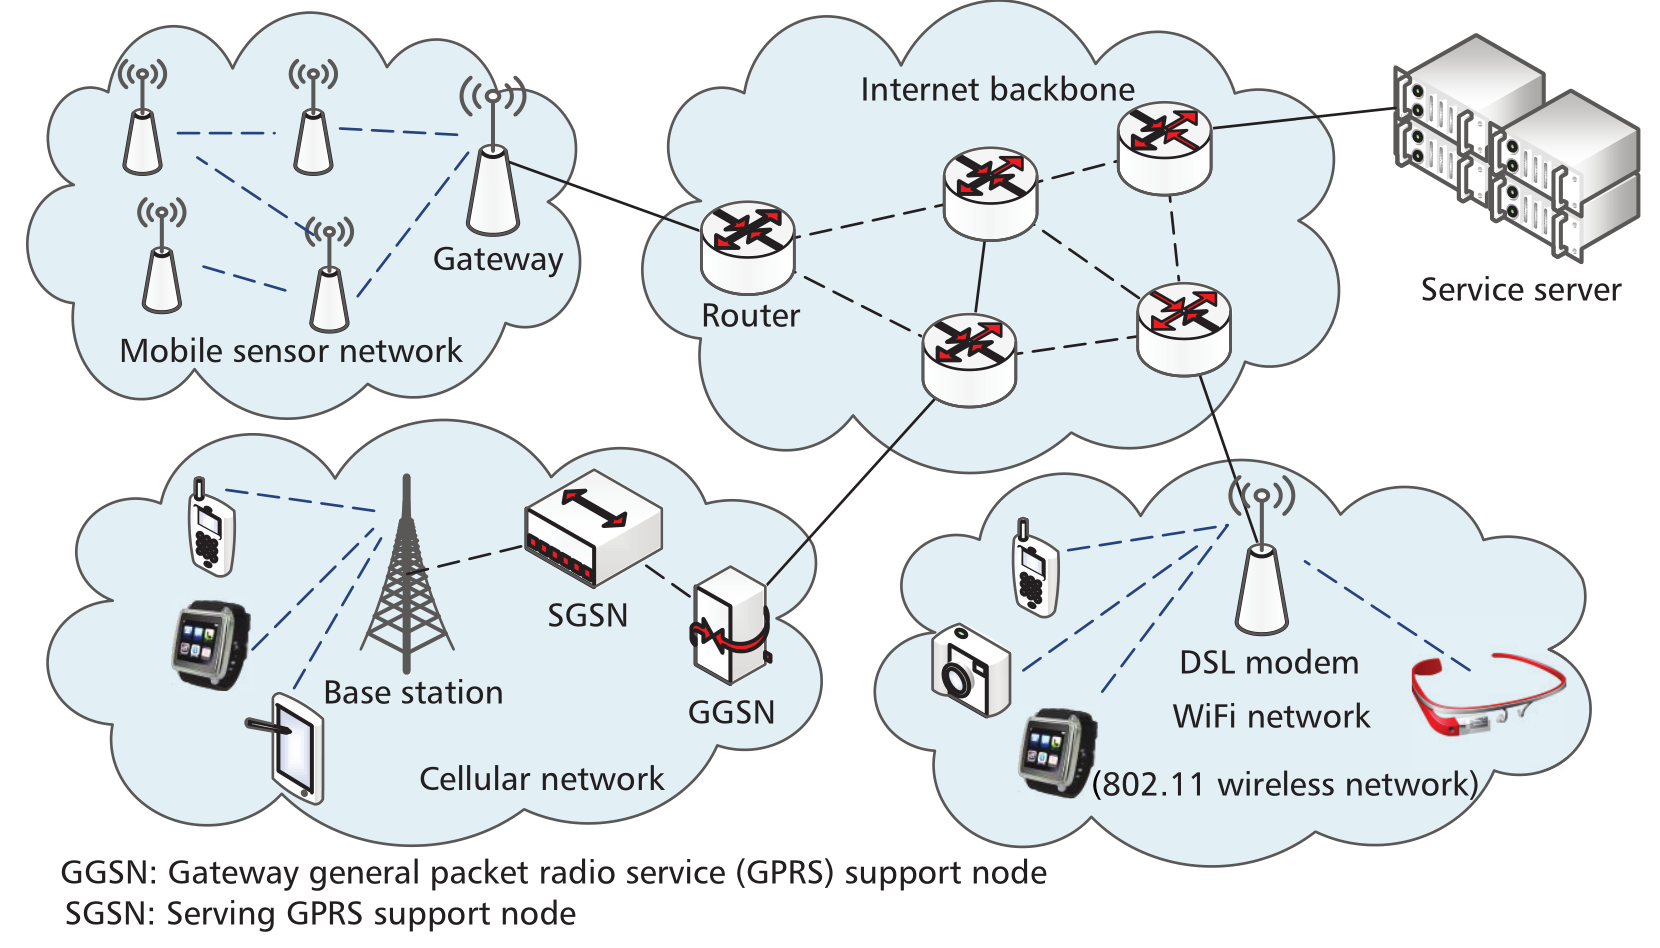
\includegraphics[width=.8\linewidth]{mbd_architecture.png}
    \caption{Illustration of the MBD era: typical architecture of a modern mobile network connecting smartphones, wearable
computers, and IoT gadgets.}
\end{figure}

MBD analytics is more versatile than conventional big
data problems as data sources are portable and data traffi c is
crowdsourced. MBD analytics deals with massive amounts of
data collected by millions of mobile devices. Next, we discuss
the main characteristics of MBD that complicate data analytics
and learning on MBD compared to small datasets.

\subsection{Challanges of MBD Analytics}

Figure 2 shows the main recent technologies that have pro-
duced the challenging MBD era: large-scale and high-speed
mobile networks, portability, and crowdsourcing. Each tech-
nology contributes to forming the MBD characteristics in the
following ways.

\begin{figure}[!h]
	\centering
    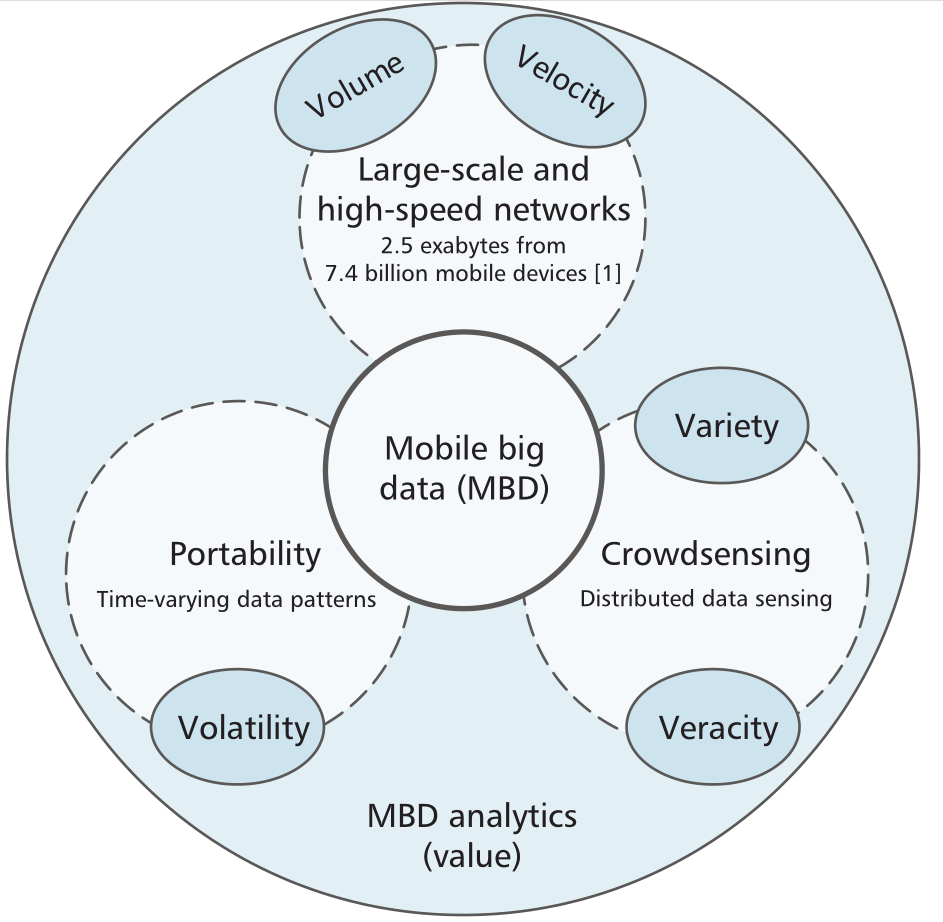
\includegraphics[width=.8\linewidth]{mbd_structure.png}
    \caption{Illustration of the MBD era: typical architecture of a modern mobile network connecting smartphones, wearable
computers, and IoT gadgets.}
\end{figure}


\textbf{Large-scale and high-speed mobile networks: }The growth
of mobile devices and high-speed mobile networks (e.g., WiFi
and cellular networks) introduces massive and increasingly
contentious mobile data traffi c. This is refl ected in the follow-
ing MBD aspects:

\begin{itemize}
\item {\textit{MBD is massive (volume):} In 2015, 3.7 exabytes of mobile
data was generated per month, which is expected to increase
through the coming years }

\item{\textit{MBD is generated at increasing rates (velocity): }MBD flows
at a high rate, which impacts the latency in serving mobile
users. Long queuing time of requests results in less satisfi ed
users and increased cost of late decisions.}

\end{itemize}

\textbf{Portability:} Each mobile device is free to move inde-
pendently among many locations. Therefore, MBD is non-sta-
tionary (volatility). Due to portability, the time duration in
which the collected data is valid for decision making can be
relatively short. MBD analytics should be frequently executed
to cope with the newly collected data samples.

\textbf{Crowdsourcing:} A remarkable trend of mobile applications
is crowdsourcing for pervasive sensing, which includes massive
data collection from many participating users. Crowdsensing
differs from conventional mobile sensing systems as the sens-
ing devices are not owned by one institution but instead by
many individuals from different places. This has introduced
the following MBD challenges:

\begin{itemize}
\item {\textit{MBD quality is not guaranteed (veracity):} This aspect is critical
for assessing the quality uncertainty of MBD as mobile sys-
tems do not directly manage the sensing process of mobile
devices. Since most mobile data is crowdsourced, MBD can
contain low-quality and missing data samples due to noise,
malfunctioning or uncalibrated sensors of mobile devices,
and even intruders (e.g., badly labeled crowdsourced data).
These low-quality data points affect the analytical accuracy
of MBD.}

\item{\textit{MBD is heterogeneous (variety):} The variety of MBD arises
because the data traffi c comes from many spatially distrib-
uted data sources (i.e., mobile devices). Also, MBD comes
in different data types due to the many sensors that mobile
devices support. For example, a triaxial accelerometer gen-
erates proper acceleration measurements, while a light sen-
sor generates illumination values.}

\end{itemize}

MBD analytics (\textit{value}) is mainly about extracting knowledge
and patterns from MBD. In this way, MBD can be utilized to
provide better services to mobile users and create revenue for
mobile businesses. The next section discusses deep learning as
a solid tool in MBD analytics.

\section{Deep Learning in MBD Analytics}

Deep learning is a new branch of machine learning that can
solve a broad set of complex problems in MBD analytics (e.g.,
classification and regression). A deep learning model consists of
simulated neurons and synapses that can be trained to learn
hierarchical features from existing MBD samples. The resulting deep model can generalize and process unseen streaming
MBD samples.

For simplicity, we present a general discussion of deep
learning methods without focusing on the derivations of particular techniques. Nonetheless, we refer interested readers to
more technical papers of deep belief networks and stacked
denoising autoencoders. A deep model can be scaled to
contain many hidden layers and millions of parameters, which
are difficult to train at once. Instead, greedy layer-by-layer
learning algorithms have been proposed that basically
work as follows.

\begin{figure}[!h]
	\centering
    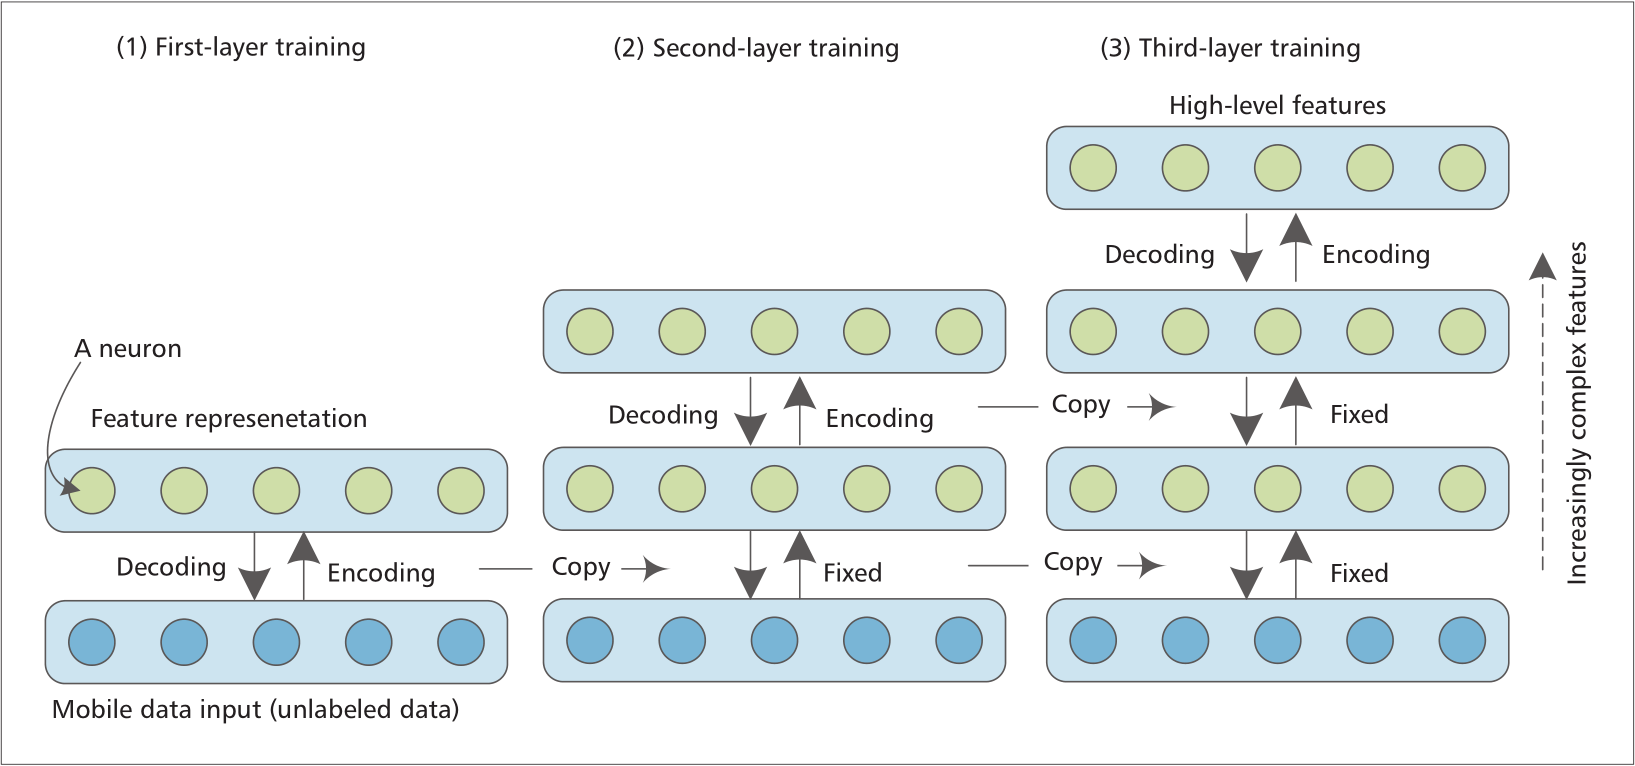
\includegraphics[width=.8\linewidth]{deep_learning.png}
    \caption{Illustration of the MBD era: typical architecture of a modern mobile network connecting smartphones, wearable
computers, and IoT gadgets.}
\end{figure}


\textbf{Generative layer-wise pre-training:} This stage requires only
unlabeled data, which is often abundant and cheap to collect
in mobile systems using crowdsourcing. Figure 3 shows the
layer-wise tuning of a deep model. First, one layer of neurons
is trained using the unlabeled data samples. To learn the input
data structure, each layer includes encoding and decoding
functions. The encoding function uses the input data and the
layer parameters to generate a set of new features. Then the
decoding function uses the features and the layer parameters
to produce a reconstruction of the input data. As a result, a
first set of features is generated at the output of the first layer.
Then a second layer of neurons is added on top of the first
layer, where the output of the first layer is fed as input of the
second layer. This process is repeated by adding more layers
until a suitable deep model is formed. Accordingly, more com-
plex features are learned at each layer based on the features
that were generated at its lower layer.

\textbf{Discriminative fine-tuning:} The model’s parameters, which
are initialized in the first step, are then slightly fine-tuned
using the available set of labeled data to solve the problem at
hand.

\subsection{Deep Learning Advantages in MBD Analytics}

Deep learning provides solid learning models for MBD analytics. This argument can be supported with the following advantages of using deep learning in MBD analytics.

\textbf{Deep learning scores highly accurate results, which are
a top priority for growing mobile systems.} Highly accurate
results of MBD analytics are required for sustainable business
and effective decisions. For example, poor fraud detection
results in expensive loss of income for mobile systems. Deep learning models have been reported as state-of-the-art methods to solve many MBD tasks.


Deep learning generates intrinsic features that are
required in MBD analytics. A feature is a measurement attribute extracted from sensory data to capture the underlying
phenomena being observed and enable more effective MBD
analytics. Deep learning can automatically learn high-level
features from MBD, eliminating the need for the handcrafted
features in conventional machine learning methods.

\textbf{Multimodal deep learning:} The “variety” aspect of MBD
leads to multiple data modalities of multiple sensors (e.g.,
accelerometer samples, audio, and images). Multimodal deep
learning can learn from multiple modalities and heteroge-
neous input signals.

\subsection{The curse of dimensionality:}

MBD comes with volume and
velocity related challenges. Historically, data analytics on small
amounts of collected data (a.k.a. random sampling) was utilized. Despite the low computational burden of random sampling, it suffers from poor performance on unseen streaming samples. This performance problem is typically avoided by
using the full set of available big data samples, which significantly increases the computational burdens.
Large-scale deep models: To fully capture the information
on MBD and avoid underfitting, deep learning models should
contain millions of free parameters; for example, a 5-layer
deep model with 2000 neurons per layer contains around 20
million parameters. Models’ free parameters are optimized
using gradient-based learning, which is computationally
expensive for large-scale deep models.
Time-varying deep models: In mobile systems, the continuous adaptation of deep models over time is required due to
the volatility characteristic of MBD.
To tackle these challenges, we next describe a scalable framework for MBD analytics using deep learning models and
Apache Spark

\section{A Spark-Based Deep Learning Framework for MBD Analytics}

Learning deep models in MBD analytics is slow and computationally demanding. Typically, this is due to the large number
of parameters of deep models and the large number of MBD
samples. Figure 3 shows the proposed architecture for learning
deep models on MBD with Apache Spark. Apache Spark
is an open source platform for scalable MapReduce computing on clusters. The main goal of the proposed framework is
speeding up MBD decision making by parallelizing the learning of deep models to a high-performance computing cluster.
In short, the parallelization of a deep model is performed
by slicing the MBD into many partitions. Each partition is
contained in a resilient distributed dataset (RDD) that provides an abstraction for data distribution by the Spark engine.
Besides data caching, RDDs of a Spark program natively support fault-tolerant executions and recover the program operations at worker nodes.


\section{Problem Statement}

Accelerometers are sensors that measure proper acceleration
of an object due to motion and gravitational force. Modern
mobile devices are widely equipped with tiny accelerometer
circuits, which are produced from electromechanically sensitive elements and generate electrical signals in response to any
mechanical motion. The proper acceleration is distinctive from
coordinate acceleration in classical mechanics. The latter measures the rate of change of velocity, while the former measures
acceleration relative to a free fall; that is, the proper acceleration of an object in a free fall is zero.

Conventional approaches to recognizing activities require
handcrafted features (e.g., statistical features), which are
expensive to design, require domain expert knowledge, and
generalize poorly to support more activities. To avoid this, a
deep activity recognition model learns not only the mapping
between raw acceleration data and the corresponding activity
label, but also a set of meaningful features that are superior to
handcrafted features.


\section{Experimental Results}



\textbf{The Impact of Deep Models:} 

\begin{figure}[!h]
	\centering
    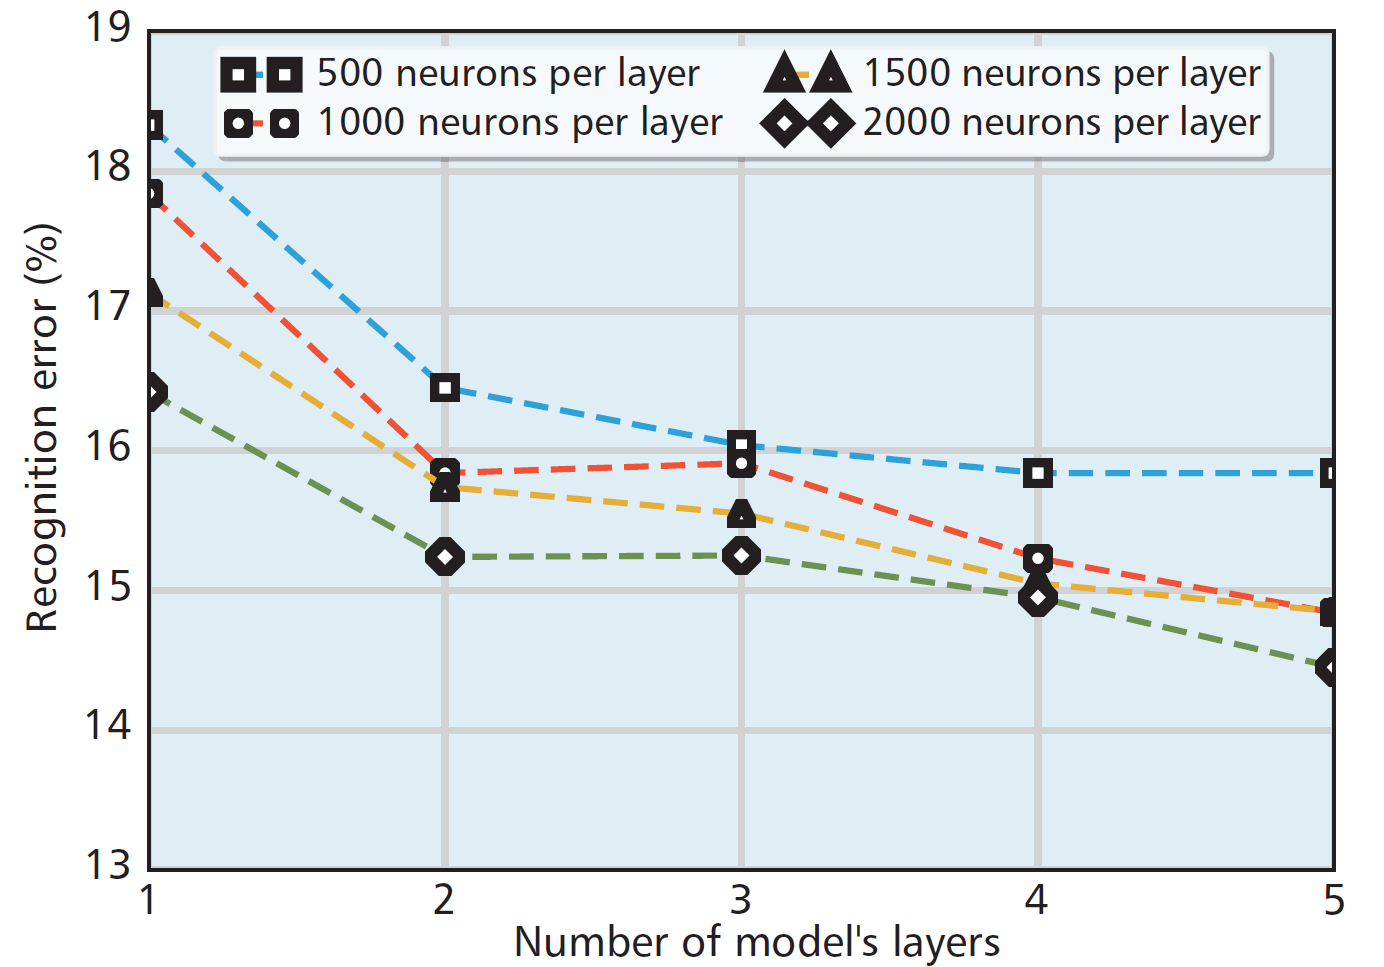
\includegraphics[width=.8\linewidth]{analysis2.png}
    \caption{Recognition accuracy of deep
learning models under different deep model setups}
	\label{fig:layer}
\end{figure}


Figure \ref{fig:layer} shows the activity rec-
ognition error under different setups of deep models (num-
ber of hidden layers and number of neurons at each layer).
Specifically, the capacity of a deep model to capture MBD
structures is increased when using deeper models with more
layers and neurons. Nonetheless, using deeper models involves
a significant increase in the learning algorithm’s computational
burdens and time. 

\textbf{The Impact of Computing Cores:} 


\begin{figure}[!h]
	\centering
    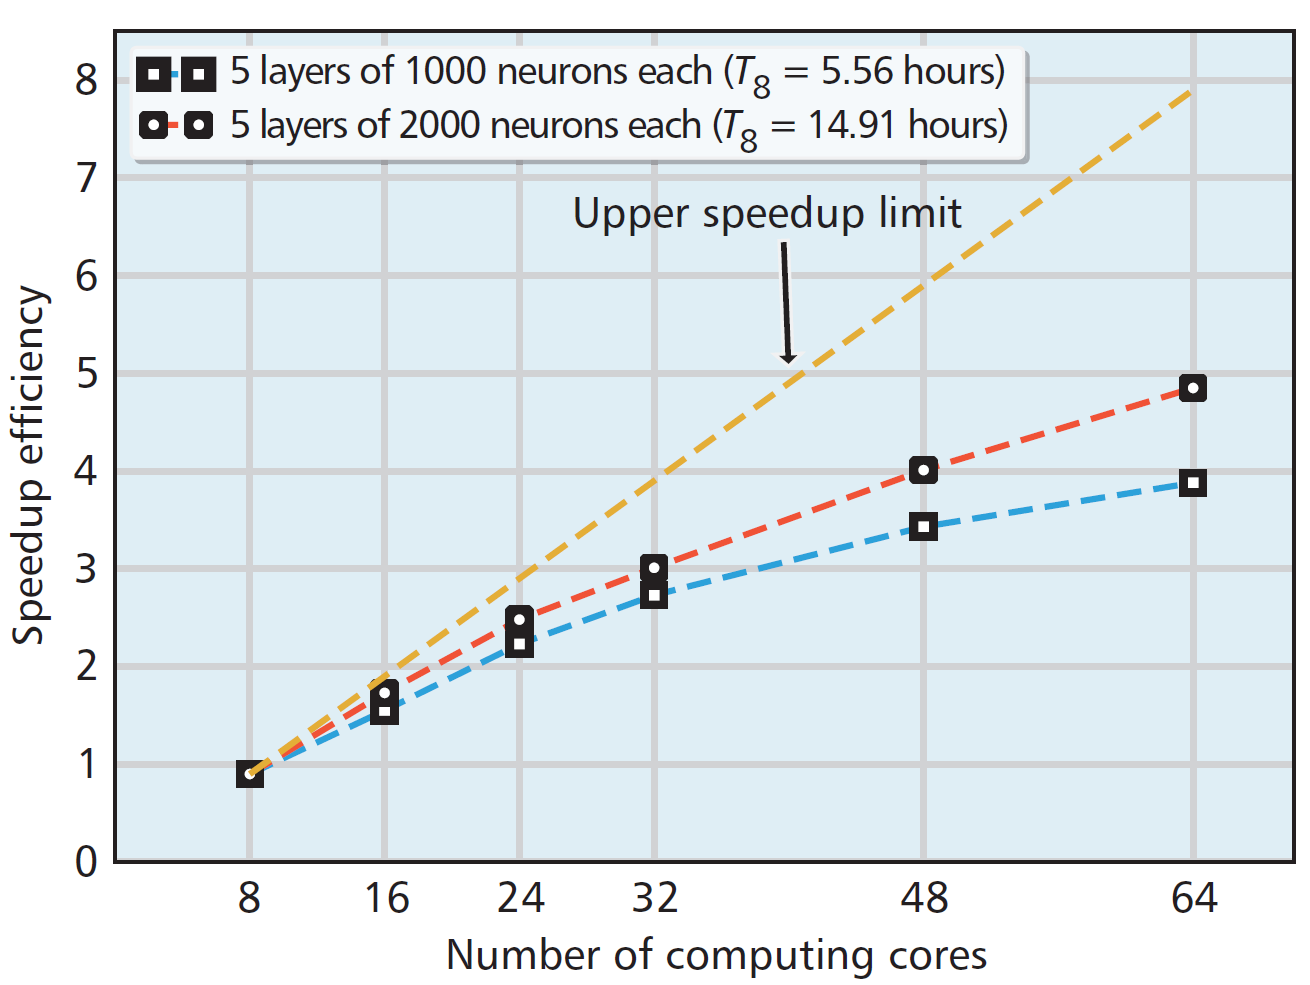
\includegraphics[width=.8\linewidth]{analysis3.png}
    \caption{Speedup of learning deep models using the Spark-based
framework under different computing cores.}
	\label{fig:core}
\end{figure}

The main performance metric
of cluster-based computing is the task speedup metric. Figure \ref{fig:core}
shows the speedup in learning deep models when the number of
computing cores is varied. As the number of cores increases, the
learning time decreases.

\newpage

\section{Conclusion}

In this article, we have presented and discussed a scalable
Spark-based framework for deep learning in mobile big data
analytics. The framework enables the tuning of deep models
with many hidden layers and millions of parameters on a computing cluster. Typically, deep learning provides a promising
learning tool for adding value by learning intrinsic features
from raw mobile big data. The framework has been validated
using a large-scale activity recognition system as a case study.
Finally, important research directions on mobile big data have
been outlined.

\end{document}